\documentclass{article}
\usepackage[T1]{fontenc}
\usepackage{lmodern}
\usepackage{graphicx}
\usepackage{amsmath,amssymb}
\usepackage[a4paper,margin=2cm]{geometry}
\usepackage[absolute,overlay]{textpos}
\setlength{\TPHorizModule}{1mm}
\setlength{\TPVertModule}{1mm}
\usepackage[indonesian]{babel}
\usepackage{hyperref}
\setlength{\emergencystretch}{2em}
% unit: Halaman 3

\begin{document}

% === Halaman 3 (llm) ===

\vspace{83.46mm}

\begin{itemize}
    \item Steganografi
\end{itemize}
\vspace{60mm}
\begin{itemize}
    \item Steganalisis
\end{itemize}
\vspace{30mm}
*) Keterangan: 1 jika ada pesan tersembunyi, 0 jika tidak

\vspace{23.76mm}

% deskripsi: Diagram proses steganografi yang menunjukkan aliran dari message dan cover-object melalui proses Embedding menggunakan key untuk menghasilkan stego-object, yang kemudian diproses oleh adversary atau di-extract menggunakan key untuk mendapatkan kembali message.
% bbox normalisasi: [0.2170, 0.2020, 0.7510, 0.4830]
\begin{textblock*}{112.14mm}(45.57mm,59.99mm)
\noindent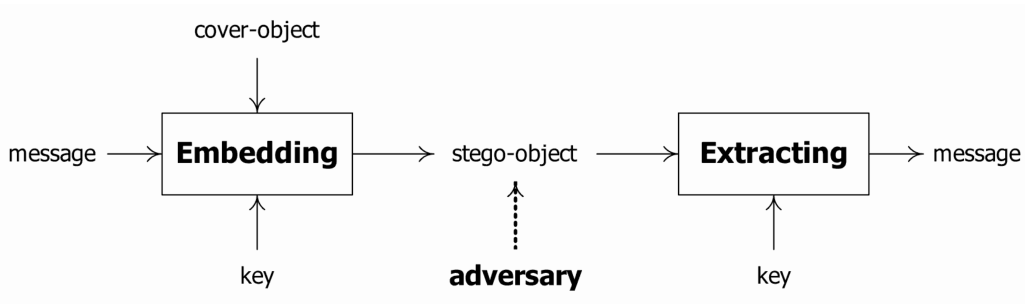
\includegraphics[width=112.14mm,height=83.46mm]{../../images/llm/page_003_img_01.png}%
\end{textblock*}

% deskripsi: Diagram proses steganalisis yang menunjukkan input berupa suspected stego object yang masuk ke blok Analisis untuk menghasilkan decision (1/0).
% bbox normalisasi: [0.2360, 0.6670, 0.6280, 0.7470]
\begin{textblock*}{82.32mm}(49.56mm,198.10mm)
\noindent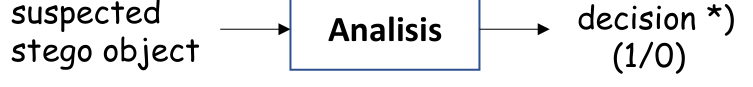
\includegraphics[width=82.32mm,height=23.76mm]{../../images/llm/page_003_img_02.png}%
\end{textblock*}

\end{document}
